\documentclass[10pt,a4paper]{scrartcl} 
\usepackage[left=1cm,right=1cm,top=1cm,bottom=1cm]{geometry} 
\usepackage[utf8]{inputenc} 
\usepackage[ngerman]{babel} 
\usepackage[most]{tcolorbox}
\usepackage[official]{eurosym}
\usepackage{amsmath}
\usepackage[bookmarks,bookmarksopen,bookmarksdepth=2]{hyperref}
\usepackage{cancel}
\usepackage{enumitem}
\usepackage{tabularx}
\usepackage{xcolor}
\usepackage{MnSymbol,wasysym}
\usepackage{tikz-timing}
\usepackage{subcaption}
\usepackage{acronym}
\usepackage{tikz, pgfplots}
\usetikzlibrary{calc}

	\usepgfplotslibrary{groupplots}

\def\doubleunderline#1{\underline{\underline{#1}}}

\def\rot{\rotatebox}


\newcommand{\tikzmark}[2]{\tikz[overlay, remember picture] \node[inner sep=0pt, outer sep=0pt, anchor=base] (#1) {#2};}

\newcommand\hcancel[2][black]{\setbox0=\hbox{$#2$}%
	\rlap{\raisebox{.45\ht0}{\textcolor{#1}{\rule{\wd0}{1pt}}}}#2} 

\newcommand{\reftbl}[1]{Tabelle ~\ref{#1}}

\tikzset{
	timing/z/.style={color=blue},
	timing/l/.style={color=blue},
	timing/h/.style={color=blue}
}

\newtcbtheorem[no counter]{Theorem}{Definition}{
	enhanced,
	sharp corners,
	attach boxed title to top left={
		yshifttext=-1mm
	},
	colback=white,
	colframe=blue!75!black,
	fonttitle=\bfseries,
	boxed title style={
		sharp corners,
		size=small,
		colback=blue!75!black,
		colframe=blue!75!black,
	} 
}{thm}
\newtcbtheorem[no counter]{Hint}{Hinweis}{
	enhanced,
	sharp corners,
	attach boxed title to top left={
		yshifttext=-1mm
	},
	colback=white,
	colframe=yellow!75,
	fonttitle=\color{black}\bfseries,
	boxed title style={
		sharp corners,
		size=small,
		colback=yellow!75,
		colframe=yellow!75,
	} 
}{thm}

\newcolumntype{Y}{>{\centering\arraybackslash}X}

\newcommand*\circled[1]{\tikz[baseline=(char.base)]{
		\node[shape=circle,draw,inner sep=1pt] (char) {#1};}}

\author{Levin Baumann}
\title{Digitaltechnik}

\begin{document}
	\maketitle
	\section{Begriffe}
	\begin{tabular}{r|l}
		digital & analog \\
		wertediskret & wertekontinuierlich\\
		$\Rightarrow$ zwischen zwei benachbarten gibt es \underline{keine} zwischenwerte & $\Rightarrow$ zwischen zwei beliebigen gibt es unendlich viele Zwischenwerte \\
		$ \Rightarrow $ endlich oder auch unendlich (aber abzählbar viele) & $ \Rightarrow $ Immer unendlich (und sogar überabzählbar) viele Werte \\
		meist zeitdiskret (\glqq getaktet\grqq) & zeitkontinuierlich \\
		$ \Rightarrow $ unsere heutigen Rechner arbeiten digital & $ \Rightarrow $ unsere Welt \glqq arbeitet\grqq\ analog
	\end{tabular}

\section{Codierung}

	\begin{Theorem}{}{fermat}
		Codierung ist die Darstellung von Informationen mit einem \glqq Alphabet\grqq.
	\end{Theorem}
		
	\begin{Theorem}{}{fermat}
		Alphabet ist eine \underline{endliche} Menge von Symbolen
	\end{Theorem}
	
	\textit{Anmerkung: Codierung ist immer mit Digitalisierung verbunden.} \\
	
	\subsection{Arten von Codierungen}
	\begin{itemize}
		\item Zeichencodierung
		\item Zahlencodierung (Text-, Bildbearbeitung,\dots)
		\item Verschlüssellung (\textit{Achtung:} Unterschied zu anderen Codierungen: Aus der codierten verschlüsselten Info sollen die meisten Menschen nicht auf die Ursprungsinfo schließen können)
		\item Signalcodierung
	\end{itemize}

	\subsection{Codierungen}
	\subsubsection{Zeichencodierung}
	\begin{itemize}
		\item ASCII: Alphabet besteht aus (ganzen) Zahlen von 0 bis 127
		\item ISO8859-x: Alphabet besteht aus 0\dots255
		\subitem -x: verschiedene Sprachräume
		\subitem -1: westeuropäisch
		\subitem -5: kyrillisch
		\subitem -7: griechisch
		\subitem -15: westeuropäisch inkl. \euro{}
		\item Unicode: Anspruch, alle (derzeitigen, künftigen, ehemaligen) Schriftsprachen abzudecken, auch Phantasiesprachen wie Klingonisch oder Elbisch
		\subitem UTF-8: 256 Zahlenwerte
		\subitem UTF-16: 65536 Zahlenwerte
		\subitem$ \rightarrow $ Zeichen werden als variabel lange Symbolfolgen dargestellt. Gesetztes MSB zeigt an, dass mindestens ein Folgesymbol folgt.
	\end{itemize}
	\subsubsection{Zahlencodierung}
	\paragraph{I. Abzählsysteme}
	\subparagraph{Fingerabzählsysteme}
	\begin{itemize}
		\item[] Alphabet = \{Finger\}
		\item[] Symbolwert (Finger) = 1
		\item[$ \ominus $] stark beschränkter Wertebereich von 0 bis 10
		\item[$ \ominus $] bis auf weiteres nur nicht-negative ganze Zahlen
		\item[$ \oplus $] extrem einfach und verständlich		
		\item[$ \oplus $] extrem einfache Addition und Subtraktion
		\item[$ \ominus $] Multiplikation und Divisionmit erhöhtem Aufwand
		\item[$ \oplus $] Immer verfügbar/\glqq zur Hand\grqq\
	\end{itemize}
	\subparagraph{Strichliste (einfache)}
	\begin{itemize}
		\item[] Alphabet = \{I\}
		\item[] Wert (I) = 1
		\item[$ \oplus $] unbeschränkter Wertebereich
		\item[$ \oplus $] Addition weiter einfach, Subtraktion braucht man eine Entfernungsmöglichkeit/Entwertungsmöglichkeit
		\item[$ \ominus $] Hilfsmittel (Schreibwerkzeug) notwendig
		\item[$ \ominus $] unübersichtlich darstellbarer Wertebereich bis etwa 10 (10 Symbole notiert)
	\end{itemize}
	\subparagraph{erweiterte Strichliste (\glqq Lattenzaunsystem \grqq)}
	\begin{itemize}
		\item[] Alphabet = {I, \cancel{\text{IIII}}}
		\item[] Wert ( I ) = 1
		\item[] Wert ( \cancel{\text{IIII}} ) = 5
		\item[] Regeln:Symbole müssen nach Wertigkeit sortiert notiert werden. Fünf einfache Striche müssen immer zu einem „Kombisymbol“ zusammengefasst werden.
		\item[$ \oplus/\ominus $] Addition etwas erschwert durch Sortieren und Zusammenfassen; Subtraktion zusätzlich erschwert durch Auflösen des Kombisymbols 
		\item[$ \oplus/\ominus $] etwas komplexer durch zweites Symbol und Sortierregel
		\item[$ \oplus/\ominus $] übersichtlich darstellbarer Wert bis etwa 50 erweitert
	\end{itemize}

	\subparagraph{römisches Zahlensystem}
	\begin{itemize}
		\item[] Alphabet = \{I, V, X, L, C, D, M\}
		\item[] Wert = \{1, 5, 10, 50, 100, 500, 1000\}
		\item[] Zusatzregel: Symbol kleinerer Wertigkeit darf vor einem Symbol größerer Wertigkeit notiert werden Sein Symbolwert wird dann subtrahiert, statt addiert. Mehr als drei gleiche Symbole sind nicht hintereinander erlaubt 
		\item[$ \oplus/\ominus $] übersichtlich darstellbarer Wertebereich bis etwa 10.000 (?)
		\item[$ \ominus $] beschränkter Wertebereich bis < 4000
		\item[$ \ominus $] recht hohe Komplexität, relativ geringe Verständlichkeit
		\item[$ \ominus $] extrem komplizierte Addition und Subtraktion
	\end{itemize}
	\paragraph{II. \acp{SWS}}
	\subparagraph{Dezimalsystem}
	\begin{itemize}
		\item[] Alphabet = \{0, 1, 2, 3, 4, 5, 6, 7, 8, 9\}
		\item[] Symbole werden auch Ziffern genannt
		\item[] Zahl ist notiert als Folge von Ziffern: z.B. 4711
		\item[] Ziffernwert = Symbolwert
		\item[] Ziffernwert (4) = 4
		\item[] Zahlenwert = Summe (Ziffernwert * Stellenwert) 
		\item[] Stellenwert (rechte Ziffer) = 1  
		\item[]Stellenwert wächst mit jeder Stelle nach links um Faktor 10
	\end{itemize}
	$$
	Wert(Z_{n-1} \dots Z_0) = \sum_{i=0}^{n-1}|Z_i|\cdot10^i
	$$
	\subparagraph{\ac{SWS} zur Basis b}
	\begin{itemize}
		\item[] Alphabet enthält b Ziffern
		\item[] Alphabet beginnt bei Ziffer \glqq 0\grqq\ und endet bei Ziffer \glqq b-1\grqq\
	\end{itemize} 
	$$
		Wert(Z_{n-1} \dots Z_0) = \sum_{i=0}^{n-1}|Z_i| \cdot b^i
	$$
	$b_{EIN}$ mit $b>1$\\
	\textit{Anmerkung:} $b=1$ nicht sinnvoll, da im \ac{SWS} zur Basis nur die 0 dargestelt werden könnte.
	\begin{itemize}
		\item[$ \oplus/\ominus $] gewisses \glqq Erstverständnis \grqq\/Lernaufwand ist nötig
		\item[$ \oplus/\ominus $] es gibt für jede Grundrechenart einVerfahren mit etwas erhöhter Komplexität, welches aber nach erstmaligem Lernaufwand doch relativ problemfrei realisierbar ist
		\item[$ \oplus/\ominus $] unbeschränkter Wertebereich
		\item[$ \oplus/\ominus $] Wertebereich bis etwa $b^10$ ist übersichtlich darstelbar
	\end{itemize}
	\subsubsection*{Umrechnung}
	\begin{itemize}
		\item Von Basis $b$ nach Basis $10$?
		\subitem $\Rightarrow$ Werteformel
		\item Von Basis $10$ nach Basis $ b $?
		\subitem $ \Rightarrow $ Werteformel umgekehrt
		\subitem $ \Rightarrow $ Ganzzahldivision
	\end{itemize}
	\begin{equation}
	\begin{split}
	{42}_{10} &= 101010\\	
	43:2 &= 21R0 = Z_0\\
	21:2 &= 10R1 = Z_1\\
	10:2 &= 5R0 = Z_2\\
	5:2  &= 2R1 = Z_3\\
	2:2  &= 1R0 =Z_4\\
	1:2	&= 0R1 = Z_5
	\end{split}
	\end{equation}
	Hinweis: Führende \glqq 0 \grqq\ können bei Zahlen im \ac{SWS} beliebig hinzugefügt oder weggelassen werden. 
	allg: Umrechnung von Basis $b_1$ nach Basis $b_2$
	\begin{itemize}
		\item meist: von Basis $b_1$ nach $b_Z=10$ dann von $b_Z$ nach $b_2$
		\item theoretisch: Ganzzahldivision durch Zielbasis $b_2$, aber ausgeführt im \ac{SWS} zur Ausgangsbasis $\Rightarrow$ Nicht praktikabel
	\end{itemize}
	Direkte Umrechnung:\\
	Falls $ b_1 = {b_2}^n $, dann entsprechen $n$ Ziffern zur Basis $ b_2 $ einer Ziffer zur Basis $ b_1 $ und es ist eine ziffern(block)weise Umrechnung.\\
	\\
	\underline{Bsp.:} $ b_1=2 $ und $ b_2=16 $\\
	$ \Rightarrow $ 4 Ziffern zur Basis $ 2 $ entsprechen einer Ziffer zur Basis $ 16 $.\\ \\
	
	\underline{Gängige Basen im \ac{SWS}}\\
	$ b=10 $ \glqq Dezimalsystem\grqq\ $ \Rightarrow $ Mensch\\
	$ b=2 $ \glqq Binärsystem\grqq\/\glqq Dualsystem\grqq\ $ \Rightarrow $ Digitalrechner \\
	$ b=16 $ \glqq Hexadezimalsystem \grqq\ $ \Rightarrow $ Computernahe Darstellung von Zahlen
	\begin{itemize}
		\item weniger Stellen
		\item einfache Umrechnung
	\end{itemize}
	$ b=8 $ \glqq Oktalsystem\grqq\ $ \Rightarrow $ Computernahe Darstellung von Zahlen\\
	$ b=16 $ vs. $ b=8 $ nur \glqq normale\grqq\ Zahlen notwendig
	
	\subsubsection*{Hexadezimalsystem}
	\begin{tabular}{ccc}
		Wert & Ziffer & Binär\\
		0 & 0 & 0000\\
		1 & 1 & 0001\\
		2 & 2 & 0010\\
		3 & 3 & 0011\\
		4 & 4 & 0100\\
		5 & 5 & 0101\\
		6 & 6 & 0110\\
		7 & 7 & 0111\\
		8 & 8 & 1000\\
		9 & 9 & 1001\\
		10 & 10 & 1010\\
		11 & 11 & 1011\\
		12 & 12 & 1100\\
		13 & 13 & 1101\\
		14 & 14 & 1110\\
		15 & 15 & 1111\\
	\end{tabular}
\begin{minipage}[b]{0.7\textwidth}
	\centering
	BSP: $ABEF_{16}$
	$$
	\begin{array}{c|c|c|c}
	1010 & 1011 & 1110 & 1111
	\end{array}
	$$
	\\
	$$
	\begin{array}{c|c|c|c|ccc}
	0001&1001&0001&1100 & 0101_2 & = & 191C5_{16}\\
	1 & 9 & 1 & C & 5 & 
	\end{array}$$
\end{minipage}%
\\
\\
Falls $b_1^n = b_2^m$, dann entspricht ein Ziffernblock von $n$ Ziffern zur Basis $b_1$ einem Ziffernblock von $m$ Ziffern zur Basis $b_2$.
\\
$$
\begin{array}{rcl}
2^{3n} = 2^{4m} & \Rightarrow & n=4 \& m=3\\
				& \Rightarrow & \textrm{4 Ziffern zur Basis 8 entrsprechen}\\
				&             & \textrm{3 Ziffern zur Basis 16 entrsprechen}\\
				&             & \textrm{Problem: Tabelle hat } 2^{12} \textrm{ Zeilen}\\
\end{array}
$$

\subsubsection*{Einschränkungen aufheben}
\hspace*{2em}
auch negative Zahlen!
\\
\subsection{Darstellung negativer Zahlen}
 Vorzeichen und Betrag
\subsubsection{1er-Komplement}
	\textit{(ab jetzt immer zur Basis 2)}\\
	Alle Bits werden invertiert: $ 0 \rightarrow 1; \; 1\rightarrow 0 $\\
	Aber vorher: bei positiven Zahlen mindestens eine führende Null.\\
	Außerdem: alle Zahlen auf \underline{gleiche} Länge!

$$
\begin{array}{rc}
	& 42 \\
 -  & 37 \\
    & \\
    &
\end{array}
\begin{array}{cccccccccl}
       & 0 & 0 & 1 & 0 & 1 & 0 & 1 & 0 &\\
       & 1 & 1 & 0 & 1 & 1 & 0 & 1 & 0 &\\
 _1 & _1 & _1 & _1 & _1 &     & _1 &    & &\\ \hline
\hcancel[red]{1}  & 0 & 0 & 0 & 0 & 0 & 1 & 0 & 0 & \text{(9. Stelle wird ignoriert)}

\end{array}
$$

\subsubsection*{Nachteile 1er-Komplement}
\begin{itemize}
	\item Manchmal (leicht) falsche ERgebnisse
	\item Zwei verschiedene Darstellungen der \glqq 0\grqq \\
	$  +0 \hat{=} 0000 \xrightarrow{e.K.} 1111 \hat{=} -0 $
\end{itemize}
\subsubsection*{Wertebereich 8bit-1-IC-Zahlen:}
$$
01111111 = 127 \\
-127 = 10000000 \xrightarrow{eK} 01111111 = 127
$$
$\Rightarrow$ nur 255 (statt $ 256 = 2^8 $) verschiedene Zahlenwerte mit 8 Bit darstellbar

\subsubsection{2er Komplement}
Bildung: Wie 1er-Komplement, also Stellenzahl festlegen, Ziffern invertieren ($ 0 \rightarrow 1; \; 1\rightarrow 0 $)\\
\textbf{Zusätzlich:} +1 addieren!\\
\\
$ \bigoplus $ Ergebnis immer korrekt!

\subsection{Darstellung nicht-ganzer (aber vorläufig nicht-negativer) Zahlen}
\subsubsection{Bruch: Darstellung mit Zähler \& Nenner}
$$
\dfrac{1}{2} = \dfrac{2}{4} \\
\dfrac{1}{4}
$$

$ \bigominus $ Es gibt unendlich viele Darstellungen jeder Zahl als Bruch. Lösungsmöglichkeit: nur gekürzte Darstellung.\\
$ \Rightarrow $ Normalerweise keine Darstellung von Zahlen als Bruch im PC (Ausnahme: algebraisches Lösen von Gleichungssystemen)

\subsubsection{\acp{FKZ}}
Alphabet mit Ziffern wird erweitert um \glqq Komma \grqq (\glqq , \grqq)\\
$ \Rightarrow $ In der Symbolfolge ist maximal ein komma erlaubt. \\
Bsp: Zahl mit $n$ Vor- und Nachkommastellen
$$
Z_{n-1} Z_{n-2}\ldots Z_2 Z_1 Z_0,Z_{-1} Z_{-2} \ldots Z_{-m+1} Z_{-m+2}
$$
$$
\sum_{i=0}^{n-1} |z_i|\cdot b^i
$$

$$
\begin{array}{rrcl}
z.B. & 110,011_2 & = & 0 \cdot 2^0 + 1 \cdot 2^1 + 1 \cdot 2^2 \\
        &                     & = & 0 \cdot 2^{-1} + 1 \cdot 2^{-2} + 1 \cdot 2^{-3} \\
        &                     & = & 2 + 4 + \dfrac{1}{4} + \dfrac{1}{8} = 6 + 0,25 + 0,125 = 6,375 \\
\end{array}
$$
\\
Umrechnung von Basis 10 nach Basis b? \\
$\rightarrow$ Werteformel\\
$ z.B. 6,375_{10} = ?,?_2 $\\
\noindent
Aufteilung in Vor- und Nachkommateil: \\
Vorkommateil über Ganzzahldivision\\
$ 6_{10} = 110_{2} $\\
Nachkommateil: Multiplikation mit Zielbasis und Aufteilen in Vor- und Nachkommateil \\
Vorkommateil ist die erste bzw. nächste Nachkommastelle
$$
\begin{array}{rlcl}
0,375 & \cdot 2 & = & 0,75\\
0,75   & \cdot 2 & = & 1,5\\
0,5     & \cdot 2 & = & 1,0\\
0,0     & \cdot 2 & = & 0,0\\
\end{array}
$$
$$
0,375_{10} = 0,01100_{2}
$$

\subsubsection{\acp{GKZ}(auch Fließkommazahlen)}
$$
\text{Wert} = \text{Mantisse} \cdot \text{Basis}^{\text{Exponent}}
$$
\begin{tabular}{rl}
	Mantisse  & Festkommazahl \\
	Exponent & ganze Zahl, steht für die Verschiebung des Kommas bei der Mantisse\\
	Basis b     & beliebig (wie bei anderen Zahlen im \ac{SWS}), aber $b$ muss der für die Mantisse verwendeten Basis entsprechen\\
\end{tabular}

$$
1,0 \cdot 10^0 = 10,0 * 10^{-1} = 100,0 \cdot 10^{-2} = 0,1 \cdot 10^{1} \ldots
$$

%ToDo Rest aus Tablet übernehmen

\section{Signalkodierung}

\begin{Theorem}{}{fermat}
	Darstellung von abstrakten Informationen als Signalfolge. \\
	Signal: physisch messbare Größe.
\end{Theorem}

\subsection{mögliche Signalformen}
\begin{itemize}
	\renewcommand\labelitemi{--}
	
	\item elektrisch\\
		Spannung, Stromstärke, elektromagnetische Wellen, Ladung
	\item optisch\\
		Helligkeit, Farbe
	\item akustisch
		Lautstärke, Tonhöhe
	\item Druck
		hydraulisch, pneumatisch
\end{itemize}

\subsubsection*{in der Computertechnik relevant:}

\begin{list}{}{}
	\item[] optisch $\Rightarrow$ für netzwerkschnittstellen
	\item ekeltrisch $\Rightarrow$ insbesondere in der Digitaltechnik
	\subitem \textbf{vor allem:} Spannung (evtl. auch Stromstärke)\\
	\hspace*{2em}$\Rightarrow$ eher kleinere Spannungspegel in der Digitaltechnik
\end{list}

\subsubsection*{Strom Vs. Spannung}
\begin{figure}
	\centering
	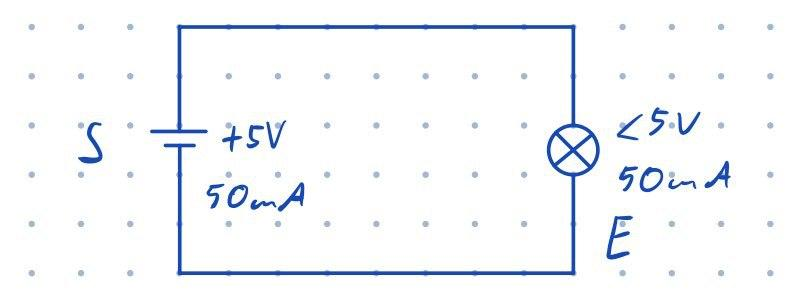
\includegraphics[width=0.5\linewidth]{img/strom_spannung_signale}
	\caption{Schaltplan mit Spannungsquelle und Glühbirne}
	\label{abb:schaltplan}
\end{figure}

\begin{tabularx}{\linewidth}{r X}
	Spannung: & Verringert sich beim E durch Spannungsfall auf der Leitung, wird verändert durch Störungen von außen (\glqq Übersprechen\grqq\, elektromagnetische Einstrahlungen)\\
	Strom: & Kaum davon betroffen; Stromstärke verändert sich im geschlossenen Stromkreis nicht.\\
\end{tabularx}
\\
Nachteil Strom: hoher Energieaufwand, große Wärmeentwicklung\\
\hspace*{2em}$\Rightarrow$ deshalb Spannung statt Strom bei den meisten Computerschnittstellen verwandt.
\\

\subsection*{typische Spannungspegel:}
\hspace*{3em}
$ \left.  \begin{array}{ccc}
0 & \hat{=} & 0V \\
1 & \hat{=} & 5V
\end{array} \right\rbrace 
$ TTL-Pegel
\\\\
\glqq Transistor-Transistor-Logic\grqq \\
\hspace*{2em} $\Rightarrow$ \glqq erfunden\grqq um 1960 von TI (TexasInstruments)

\subsubsection*{große vs. kleine Spannungspegel}

\begin{itemize}
	\item[$\bigominus$] größere sind stromanfällig bei kleineren Spannungen
	\item[$\bigoplus$] viel weniger Energieaufwand bei kleinen Spannungen, also auch weniger Wärmeentwicklung
	\item[$\bigoplus$] weniger Störauswrkungen bei kleineren Spannungen
	\item[$\bigoplus$] schnelleres Spannungswechseln bei kleinen Spannungshüben möglich
\end{itemize}

\subsection{Umsetzung von Bitfolgen in Spannungspegelfolgen}
\hspace*{2em} meist getaktet, d.h. festes Zeitraster für die Bitfolge, d.h. jedes Bit braucht eine konstante, gleichlange zeitdauer



\subsubsection*{4 Verfahren (1-4) und 4 Eigenschaften(a-d)}

\begin{enumerate}
	\item[a)] \ac{TRG}\\
	Möglichkeit, nur aus dem übertragenen Datensignal eine Resynchronisierung biem Empfänger auf den Takt des Senders zu machen
	
	\item[b)] \ac{GSF} \\
	Motivation: Einsparung der Masseleitung. Im zeitlichen Mittel liegen auf der Signalleitung 0V an.\\
	Ziel: Anhand des mittleren Signalpegels soll der Massepegel \glqq errechnet\grqq\ werden.\\
	\subitem -Vermeidung einer Potentialverschiebung beim E.
	\subitem -Pseudoargument: keine Energieübertragung beim vom S zum E.\\
	Grundvoraussetzung: symmetrische Pegel statt single-ended. \\
	z.B. $1V \hat{=} +5v$ und $0 \hat{=} -5V$\\
	dann: \ac{GSF} bei \ac{NRZ}: falls \#\glqq0\grqq\ = \#\glqq1\grqq\ (bzw. \glqq1\grqq\ und \glqq0\grqq\ im Datenstrom gleichverteilt)\\\\
	Bei den meisten Anwendungs-, Zeichen- und Zahlencodierungen kann keine Gleichverteilung angenommen werden. Ausnahme: Verschlüsselung und Kompression.
	\item[c)] \ac{SSH}\\
	(Un-)Anfälligkeit eines Verfahrens ggü. Störungen, welche durch Spannungsschwankungen auf der Leitung verursacht werden.\\
	$\Rightarrow$ direkt abhängig von der Anzahl der verwendeten Pegel, welche auf einen vorgegebenen Potentialbereich verteilt werden müssen (und so natürlich auch beim Empfänger voneinander unterschieden werden müssen)\\
	\ac{SSH} bei \ac{AMI}: schlecht, da 3 Pegel\\
	\ac{SSH} bei \ac{NRZ} und \ac{RZ}: gut, da \glqq nur\grqq\ 2 Pegel (und weniger Pegel geht nicht \smiley{})
\end{enumerate}

\begin{enumerate}
	\item \ac{NRZ}\\
		Während der gesamten Schrittdauer wird der Pegel angegegt, welcher dem zu übertragenen Bitwert entspricht
	\item \ac{RZ}
		Jeder Schritt wird in zwei Schrittzeithälften eingeteilt. Während der ersten Hälfte wird der Pegel eingenommen, welcher den zu übertragenden Bitwert entspricht und während der zweiten Hälfte immer der \glqq0\grqq\-Pegel.
		\subitem \ac{TRG} bei \ac{RZ}: Bei jeder \glqq1\grqq\ möglich, dann bei einer \glqq1\grqq\ zu Beginn und in der Mitte der Schrittzeit ein Pegelwechsel stattfindet
	\item \ac{AMI}\\
		Ähnlich \ac{NRZ} mit single-ended Pegeln, d.h. \glqq0\grqq\ wird immer mit $0V$ (während der gesamten Schrittzeit) übertragen, aber \glqq1\grqq\ abwechselnd mit z.B. $+5V$ und $-5V$ (während der gesamten Schrittzeit)
		\subitem \ac{GSF} bei \ac{AMI}: nachjeder 2. \glqq1\grqq: In der Praxis ist der GS-Anteil nach der ungeraden \glqq1\grqq\ vernachlässigbar (bei langer Übertragungszeit und vielen übertragenen \glqq1\grqq), also praktisch immer \ac{GSF}.
		\subitem \ac{TRG} bei \ac{AMI}: bei jeder \glqq1\grqq\ nur bei langer Folge von \glqq0\grqq\ keine \ac{TRG} möglich
	\item Manchester\\
		Bitwert wird über Spannungswechsel in der Mitte der Schrittzeit dargestellt, z.B. steigende Flanke $\hat{=}$ \glqq1\grqq und fallende Flanke $\hat{=}$ \glqq 0 \grqq.\\
		ggf. ist ein weiterer Spannungswechsel zu Beginn der Schrittzeit notwendig, um den nachfogenden (inhaltsführenden) Spannungswechsel durchführen zu können.
		\subitem \ac{TRG} bei Manchester: bei jedem Schritt möglich, da immer Regelwechsel in der Mitte der Schrittzeit.
		\subitem \ac{GSF} bei Manchester: immer, da sich die Pegel in erster und zweiter Schrittzeithälfte gegenseitig ausgleichen
		\subitem \ac{SSH} bei Manchester: optimal, da \glqq nur \grqq 2 Pegel
\end{enumerate}

\begin{figure}[h]
	\centering
	\begin{tikztimingtable}[timing/slope=0, scale=4]
		Data    	&  \\
		\ac{NRZ}     	& ZHZHZHZZZZHHHHH \\
		\ac{RZ} 		    & ZhzZhzZhzZZZZhzhzhzhzhz\\
		\ac{AMI}        	& ZHZLZHZZZZLHLHL \\
		Manchester 	& hzzhhzzhhzzhhzhzhzhzzhzhzhzhzh\\
		\extracode
		\makeatletter
		\tikzset{
			timing/z/.style={color=red},
			timing/l/.style={color=red},
			timing/h/.style={color=red}
		}
		\begin{pgfonlayer}{background}
			\foreach [count=\x] \b in {0,1,0,1,0,1,0,0,0,0,1,1,1,1,1} {
				\node [below,font=\sffamily\bfseries\tiny,inner ysep=2pt] at (\x-.5,.5) {\b};
			}
			\vertlines[help lines, black]{}
			\horlines[black,yshift=1.25mm]{}
		\end{pgfonlayer}
	\end{tikztimingtable}
\caption{Pegelgraphen der einzelnen Verfahren}
\end{figure}

\subsubsection*{Bandbreitenbedarf, bandbreitenbegrenzte Übertragungskanäle}
	\textbf{Nyquist-Theorem:} Über einen Übertragungskanal mit beschränkter Bandbreite kann maximal mit der Schrittrate übertragen werden, welche der doppelten Bandbreite entspricht.\\
	\textbf{\ac{BBB}: }notwendige Bandbreite für ein bestimmtes Signalcodierungsverfahren bei einer bestimmten vorgegebenen Schrittrate\\
	\textbf{\ac{BBB} bei \ac{NRZ}:} halbe Schrittrate, d.h. optimal H. Nyquist (max Frequenz bei \glqq010101...\grqq)\\
	\textbf{\ac{BBB} bei \ac{RZ}:} Schrittrate, d.h. doppelt so viel wie nötig. (max Frequenz bei \glqq000000...\grqq, oder \glqq 111111...\grqq )\\
	\textbf{\ac{BBB} bei \ac{AMI}:} halbe Schrittrate (max Frequenz bei \glqq 111111...\grqq)\\
	\textbf{\ac{BBB} bei Manchester:} Schrittrate (max Frequenz bei \glqq 000000...\grqq oder \glqq 111111 \grqq)\\

\begin{tabularx}{\textwidth}{l|Y|Y|Y|Y}
	 & \ac{TRG} 
	 & \ac{GSF} \newline symm. Pegel als Grundvoraussetzung 
	 & \ac{SSH} \newline abhängig von Anzahl Pegel 
	 & \ac{BBB} \newline abhängig von Schrittrate \\ \hline \rule{0pt}{2em} 
	 \ac{NRZ} 
	 & bei \glqq 01 \grqq und \glqq 10 \grqq \newline \circled{$=$} 
	 & \#\glqq 1 \grqq = \# \glqq 0 \grqq \newline (1 und 0 gleichverteilt) \newline \circled{$-$}
	 & 2 \newline \circled{$+$}
	 & halbe \newline \circled{$+$}\\ \hline \rule{0pt}{2em}
	 \ac{RZ}
	 & bei jeder \glqq 1 \grqq \newline \circled{$-$}
	 & symm. Pegel \& nur \glqq 1 \grqq, single ended \& nur \glqq 0 \grqq, \#1 = \#0 und umgekehrt \newline \circled{$=$}
	 & 2 \newline \circled{$+$}
	 & ganze \newline \circled{$-$} \\ \hline \rule{0pt}{2em}
	 \ac{AMI}
	 & bei jeder \glqq 1 \grqq \newline \circled{$-$}
	 & nach jeder zweiten \glqq 1 \grqq, in der Praxis \glqq immer \grqq \newline \circled{$+$}
	 & 3 \newline \circled{$-$}
	 & halbe \newline \circled{$+$} \\ \hline \rule{0pt}{2em}
	 Manch. 
	 & immer \newline \circled{$+$}
	 & immer \newline \circled{$++$}
	 & 2 \newline \circled{$+$}
	 & ganze \newline \circled{$-$} \\
\end{tabularx}
\\ \\
\textbf{Einsatz:}\\
\begin{itemize}
	\item \ac{NRZ} für interne Schnittstellen, bei denen der Verzicht auf Takt- oder Masseleitung nicht relevant ist
	\item Manchester gerne für Netzwerkschnittstellen (z.B. Ethernet) um auf Takt- und Masseleitung verzichten zu können
\end{itemize}

\subsubsection*{3 Verfahren zur sicheren Taktrückgewinnung:}
\begin{enumerate}
	\item \textbf{Startbitsequenz} \\
	Vor $n$ Nutzdatenbit wird eine Startbitsequenz gestellt, welche sichere \ac{TRG} ermöglicht. z.B. bei \ac{NRZ}: \glqq 01\grqq oder \glqq 10 \grqq. $n$ ist abhängig von der Genauigkeit der Uhren. \\
	\textbf{Nachteil:} relativ großer Overhead, effektive Nutzdatenrate deutlich kleiner als die Schrittrate.\\
	\noindent\hspace*{2em}% 
	Im Beispiel: Nutzdatenrate = $\dfrac{n}{n+2}\cdot Schrittweite$\\
	Bsp: bei \ac{RZ} oder \ac{AMI} reicht ein einfaches \glqq 1 \grqq-Startbit. (Keine \glqq Sequenz\grqq, weniger Overhead)\\
	\textbf{Anwendung:} z.B.serielle Schnittstelle RS232
	
	\item \textbf{Bitstuffing (\glqq Bitstopfen\grqq)}\\
	Nach jeweils $n$ gleichen direkt aufeinanderfolgenden Bitwerten wird ein Bit mit dem eingesetzten Bitwert eingefügt. \\
	z.B. n=3:\\
	\noindent\hspace*{3em}% 
	\begin{tabularx}{10em}{ccccccccccccccc}
		0 & 0 & 1 & 1 & 1 & 0 & 0 & 0 & 0 & 1 & 1 & 1 & 1 & 1 & 1\\
		1 & 2 & 1 & 2 & \tikzmark{stuffing1}{3}& 1 & 2 & \tikzmark{stuffing2}{3} & 1 & 1 & 2 & \tikzmark{stuffing3}{3} & 1 & 2 & \tikzmark{stuffing4}{3}\\
	\end{tabularx}
\tikz[overlay,remember picture] {
	\draw[<-,red] ($(stuffing1)+(0.3,0.3)$) -- ++(-90:0.5cm) node[below]{0};
	\draw[<-,red] ($(stuffing2)+(0.3,0.3)$) -- ++(-90:0.5cm) node[below]{0};
	\draw[<-,red] ($(stuffing3)+(0.3,0.3)$) -- ++(-90:0.5cm) node[below]{0};
	\draw[<-,red] ($(stuffing4)+(0.3,0.3)$) -- ++(-90:0.5cm) node[below]{0};
}
\\ \\ \\
	\textbf{Hinweis:} Der Empfänger schaut nach $n$ gleichen Bitwerten den nächsten Bitwert an. Bei entgegengesetztem Bitwert wird dieses \glqq Stopfbit\grqq entfernt. Bei gleichem Bitwert wird ein Fehler nach oben gemeldet.\\
	\textbf{Vor-/Nachteile:} Overhead bei \ac{NRZ} im schlimmsten fall nur halb so groß wie bei der Startbitsequenz (nur eine statt zwei Schrittzeiten pro $n$ Nutzdatenbit) und im besten Fall gar kein Overhead! \\
	\textbf{bei \ac{RZ}:} nur nach $n$ \glqq 0\grqq wird eine \glqq 1 \grqq eingefügt, d.h. weniger Overhead als bei \ac{NRZ} und Bitstuffing. Verfahren ist komplex und deshalb \grqq teuer\grqq und \glqq fehleranfällig\grqq . Nutzdatenrate ist nicht konstant abhängig von Schrittrate, sondern sie variiert abhängig von den zu übermittelnden Nutzdaten (Overhead ist variabel) $\Rightarrow$ schlecht für Anwendungen mit konstanter Nutzdatenrate (z.B. PCM-kodiertes Audio)\\
	\textbf{Anwendung:} Ethernet (um Bitmuster des Frame-Delimiters \glqq 01111110\grqq auszuschließen $\Rightarrow$ nach fünf \glqq 1\grqq wird eine Stopf-\glqq 0\grqq eingeschoben)
	
	\item \textbf{Blockcodierung}\\
	Ein Block von $n$ Nutzdatenbit wird als Block von ($n+i$) zu übertragende Datenbit codiert, wobei nur solche Blöcke verwendet werden, welche sichere \ac{TRG} ermöglichen.\\
	\textbf{Nachteil:} konstant großer Overhead\\
	\textbf{Vorteil:} ggf. sind weitere positive Eigenschaften erzielbar durch geeignete Auswahl der zu verwendenden Datenblöcke bei der Übertragung (vgl. 8B10B-Codierung und \ac{GSF}!)\\
	\textbf{Anwendung:} z.B. ISDN und viele andere
\end{enumerate}

Ganggenauigkeit der Uhren und Anzahl der Schritte ohne Resynchronisierung:
\begin{center}
\begin{tikzpicture}

\draw (0,0) -- (12,0);
\draw (0,0) node[left=3pt] {S} node[left=3pt] {$ $};

\foreach \x in {0,3,6,9,12}
\draw (\x,0.25) -- (\x,-0.25);


\draw (0,-1.5) -- (12,-1.5);
\draw (0,-1.5) node[left=3pt] {E} node[left=3pt] {$ $};

\foreach \x in {0,4,8,12}
\draw (\x,-1.25) -- (\x,-1.75);

\end{tikzpicture}
\end{center}
Der Pegel wird beim Empfang in der Mitte der angenommenen Schrittzeit abgetastet.\\
$\Rightarrow$ Die erlaubte Abweichung der Uhr bei $E$ von der uhr bei $S$ ist (weniger als) eine halbe Schrittzeit. Da sowohl $S$- als auch $E$-Uhr eine Ganggenauigkeit aufweisen können, darf jede Uhr um maximal 25\% einer Schrittzeit abweichen.\\
Bsp: Bei 5\% spezifischer Ganggenauigkeit wären 5 Schirrte \glqq zu viel\grqq

\section{Boolsche Algebra}
\begin{center}
	\textit{(angelehnt an das Skript von Burkhard Stiller an der Uni Zürich \glqq Info3 Modul Schaltnetze\grqq)
}
\end{center}
Benannt nach irischem (?) Mathematiker George Boole (1815-1864)\\
Rechensystem mit bestimmten Regeln:
\begin{itemize}
\item endliche Wertemenge $W$
\item zwei zweistellige Operatoren $\bigotimes, \bigoplus$
\item Abgeschlossenheit: $\forall a, b \in W\!: \; a \otimes  b \in W, \; a \oplus b \in W$
\end{itemize}

Es gelten die 4 huntington'schen Axiome: $\forall a,b,c \in W$
\begin{itemize}
	\item[\circled{H1}] \textbf{Kommutativgesetz}\\
	$a \oplus b = b \oplus a, \; a \otimes b =  b \otimes a$
	\item[\circled{H2}] \textbf{Distributivgesetz}\\
	$a \oplus (b \otimes c) = (a \oplus b) \otimes (a \oplus c)$\\
	$a \otimes (b \oplus c) = (a \otimes b) \oplus (a \otimes c)$
	\item[\circled{H3}] \textbf{Neutrales Element:} $\exists n, e \in IV$\\
	$a \oplus n = a \;,\; a \otimes e = a $
	\item[\circled{H4}] \textbf{Inverses Element:} $\exists \overline{a} \exists IV$\\
	$a \oplus \overline{a} = e \;, \; a \otimes \overline{a} = n$\\	
\end{itemize}
\noindent
Spezialfall: Schaltalgebra\\
Wertemenge besteht aus zwei Werten:
$IV = \{0,1\} = \{false, true\} = \{falsch, wahr\} = \{off, on\} = \{aus, an\}$\\
\begin{tabular}{rrl}
	Operatoren: & statt $\bigoplus$: & $\vee, \; ODER, \; OR\; (,\;+)$\\
	& statt $\bigotimes$:& $\wedge, \; UND, \; AND$\\
	& & (statt $a \wedge b$ geht auch $ab$)\\
	& & $\Rightarrow$ zweistellige Operatoren
\end{tabular}
\\
Durch \circled{H4} wird ein einstelliger Operator definiert:\\
\noindent\hspace*{2em}% 
$\overline{a} = \neg a \; \; NICHT, NOT$
\subsection{Schaltalgebra}
\subsubsection{Huntingtonsche Axiome in der Schaltalgebra}
\begin{itemize}
	\item[\circled{H1}] $a \vee b = b \vee a, \; a \wedge b  = b \wedge a$
	\item[\circled{H2}] $a \vee (b \wedge c) = (a \vee b) \wedge (a \vee c)$\\
	$a \wedge (b \vee c) = (a \wedge b) \vee (a \wedge c)$
	\item[\circled{H3}] $a \vee 0 = a, \; a \wedge 1 = a$
	\item[\circled{H4}] $a \vee \overline{a} = 1, \; a \wedge \overline{a} = 0$\\
	(oder: $a \vee \neg a = 1, \; a \wedge \neg a = 0$)
\end{itemize}

\subsubsection{Warum Schaltalgebra?}
$\Rightarrow$ Darstellung der zweistelligen Operatoren mit Schalttasten, wobei die Werte durch Schalter dargestellt wurden.

\begin{figure}[h]
	\centering
	\begin{subfigure}{.5\textwidth}
		\centering
		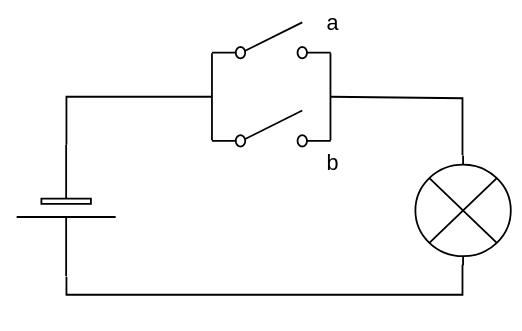
\includegraphics[width=0.8\linewidth]{img/schaltnetz_oder}
		\caption{ODER: $a \vee b$}
		\label{fig:sub1}
	\end{subfigure}%
	\begin{subfigure}{.5\textwidth}
		\centering
		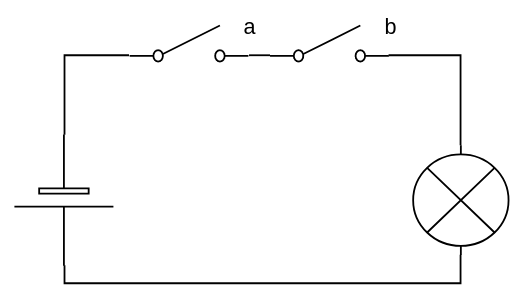
\includegraphics[width=.8\linewidth]{img/schaltnetz_und}
		\caption{UND: $a \wedge b$}
		\label{fig:sub2}
	\end{subfigure}
	\caption{Darstellung zweistelliger Operatoren mit Schaltnetzen}
	\label{fig:test}
\end{figure}

Darstellung mit Wertetabellen:\\

\begin{table}[h]
	\centering
	\begin{minipage}[b]{0.4\textwidth}
		\centering
		\begin{tabular}{cc|c|c}
			b & a & $a \vee b$ & $a \wedge b$\\ \hline
			0 & 0 & 0 & 0\\
			0 & 1 & 1 & 0\\
			1 & 0 & 1 & 0\\
			1 & 1 & 1 & 1\\
		\end{tabular}
	\end{minipage}
	\begin{minipage}[b]{0.4\textwidth}
		\centering
		\begin{tabular}{c|c}
			$a$ & $\overline{a}$\\ \hline
			0 & 1\\
			1 & 0\\
		\end{tabular}
	\end{minipage}	
	\caption{Wahrheitstabellen für UND/ODER und Negierung}
\end{table}

Ausdrücke der Schaltalgebra (\glqq boolsche Ausdrücke\grqq) bestehen aus:
\begin{itemize}
	\item ein- und zweistelligen Operatoren
	\item Variable (als Platzhalter für einen Wert)
	\item Wert
	\item Klammern
\end{itemize}
\begin{Theorem}{Eingangsbelegung}{fermat}
	Jeder Variable wird ein konkreter Wert zugeordnet
\end{Theorem}
\begin{Theorem}{Ausgangsbelegung}{fermat}
	Der Wert, welcher sich bei einem boolschen Ausdruck bei einer konkreten E-Belegung ergibt, wenn man den boolschen Ausdruck \glqq auswertet\grqq.
\end{Theorem}

Auswertung eines boolschen Ausdrucks: $(a \wedge \neg c) \vee 1 \wedge(b \wedge c) \vee (0 \wedge d)$ (Siehe \reftbl{tab:ausdruck})
\begin{itemize}
	\item Festlegung der E-Belegung
	\item Ersetzen der Variablen durch die entsprechenden Werte
	\item Auswerten \glqq von innen nach außen\grqq
	\subitem Zunächst den Teilausdruck mit der stärksten Bindungskraft, zuletzt der Teilausdruck mit der schwächsten\\ Bindungskraft: am stärksten... $NOT$, Klammer, $AND$, $OR$ ...am schwächsten
	\item bei gleicher Bindungskraft Auswertug von links nach rechts
\end{itemize}

\begin{table}[h!]
\begin{tabularx}{\textwidth}{c|cccc|Y|Y|Y|Y|Y|Y}
	\# & $ d $ & $ c $ & $ b $ & $ a $ & $ \neg c $ & $ a \wedge \neg c $ & $ 1 \wedge (b \wedge c) $ & $ 0 \wedge d $ & $ x \vee y $ & $ f $\\ \hline
	0 & 0 & 0 & 0 & 0 & 1 & 0 & 0 & 0 & 0 & 0\\
	1 & 0 & 0 & 0 & 1 & 1 & 1 & 0 & 0 & 1 & 1\\
	2 & 0 & 0 & 1 & 0 & 1 & 0 & 0 & 0 & 0 & 0\\
	3 & 0 & 0 & 1 & 1 & 1 & 1 & 0 & 0 & 1 & 1\\ \hline
	4 & 0 & 1 & 0 & 0 & 0 & 0 & 0 & 0 & 0 & 0\\
	5 & 0 & 1 & 0 & 1 & 0 & 0 & 0 & 0 & 0 & 0\\
	6 & 0 & 1 & 1 & 0 & 0 & 0 & 1 & 0 & 1 & 1\\
	7 & 0 & 1 & 1 & 1 & 0 & 0 & 1 & 0 & 1 & 1\\ \hline
	8 & 1 & 0 & 0 & 0 & 1 & 0 & 0 & 0 & 0 & 0\\
	9 & 1 & 0 & 0 & 1 & 1 & 1 & 0 & 0 & 1 & 1\\
	10 & 1 & 0 & 1 & 0 & 1 & 0 & 0 & 0 & 0 & 0\\
	11 & 1 & 0 & 1 & 1 & 1 & 1 & 0 & 0 & 1 & 1\\ \hline
	12 & 1 & 1 & 0 & 0 & 0 & 0 & 0 & 0 & 0 & 0\\
	13 & 1 & 1 & 0 & 1 & 0 & 0 & 0 & 0 & 0 & 0\\
	14 & 1 & 1 & 1 & 0 & 0 & 0 & 1 & 0 & 1 & 1\\
	15 & 1 & 1 & 1 & 1 & 0 & 0 & 1 & 0 & 1 & 1\\
\end{tabularx}
\caption{Wahrheitstabelle für $f = (a \wedge \neg c) \vee 1 \wedge (b \wedge c) \vee (0 \wedge d)$}
\label{tab:ausdruck}
\end{table}

\subsubsection{Aus den Huntingtonschen axiomen abgeleitete (beweisbare Gesetze)}
\begin{tabular}{ll}
	Assoziativgesetz & $(a \wedge b) \wedge c = a \wedge (b\wedge c)$ \\
	 & $ (a \vee b) \vee c = a \vee (b \vee c) $\\
	Idempotenzgesetz & $ a \wedge a = a $\\
	 & $ a \vee a = a $\\
	Absorptionsgesetz& $ a \wedge (a \vee b) = a $\\
    	& $ a \vee (a \wedge b) = a $\\
    DeMorgan-Gesetz  & $ \overline{(a \wedge b)} = \overline{a} \vee \overline{b} $\\
    				 & $ \overline{(a \vee b)} = \overline{a} \wedge \overline{b} $\\
\end{tabular}
\subsubsection{Beweismethoden}
\begin{itemize}
	\item algebraische Umformungen mit Hilfe der Axiome und bereits bewiesener Gesetze: \\
	$ a \overset{!}{=} a \wedge a $ (Idempotenzgesetz)\\
	$ a \overset{H3}{=} a \wedge 1 \overset{H4}{=} a \wedge ( a \vee \overline{a} ) \overset{H2}{=} (a \wedge a) \vee (a \wedge \overline{a}) \overset{H4}{=} (a \wedge a) \vee 0 \overset{H3}{=} a \wedge a$
	\item Wahrheitstabelle: Terme auf linker und rechter Seite müssen für alle Eingangsbelegugen dieselbe Ausgagsbelegung haben (\reftbl{tab:beweiswahrheitstabelle})
	\item spezielle Interpretation von $H4$:\\
	falls $ a \vee \overline{b} = 1 $ und $ a \wedge \overline{b} = 0 $, dann $ a = b $\\
	$ a \vee (b \vee c) \overset{!}{=} (a \vee b) \vee c $ (Assoziativgesetz)
\end{itemize}

\begin{table}
	\centering
	\begin{tabular}{c|ccc|c|c|c|c}
	\# & c & b & a & $ b \vee c $ & $ a \vee (b \vee c) $ & $ a \vee b $ & $ (a \vee b) \vee c$\\
	0 & 0 & 0 & 0 & 0 & 0 & 0 & 0\\
	1 & 0 & 0 & 1 & 0 & 1 & 1 & 1\\
	2 & 0 & 1 & 0 & 1 & 1 & 1 & 1\\
	3 & 0 & 1 & 1 & 1 & 1 & 1 & 1\\
	4 & 1 & 0 & 0 & 1 & 1 & 0 & 1\\
	5 & 1 & 0 & 1 & 1 & 1 & 1 & 1\\
	6 & 1 & 1 & 0 & 1 & 1 & 1 & 1\\
	7 & 1 & 1 & 1 & 1 & 1 & 1 & 1\\
	 \multicolumn{5}{c}{}& \multicolumn{1}{c}{$\uparrow$}&\multicolumn{1}{c}{}& $\uparrow$\\
	 \multicolumn{5}{c}{}&\multicolumn{3}{c}{gleiche Ausgangsbelegungen}
\end{tabular}
\label{tab:beweiswahrheitstabelle}
\caption{Beweis anhand einer Wahrheitstabelle}
\end{table}

$ \overline{a \wedge b} \overset{!}{=} \overline{a} \vee \overline{b}$\\
Beweis: 
\begin{align*}
\overline{\overline{a \vee b}}  \wedge (\overline{a} \vee \overline{b}) \overset{!}{=} 0 \\
\overline{\overline{a \wedge b}} \vee (\overline{a} \vee \overline{b}) \overset{!}{=} 1 \\
\overline{\overline{a \wedge b}} \wedge ( \overline{a} \vee \overline{b}) \overset{\text{dopp. Neg.}}{=} (a \wedge b ) \wedge (\overline{a} \vee \overline{b}) \overset{H2}{=} (a \wedge b) \wedge \overline{a} \vee (a \wedge b) \wedge \overline{b} \\
\overset{H1 \text{ \& AssG.}}{=} b \wedge (a \wedge \overline{a}) \vee a \wedge (b \wedge \overline{b}) \overset{H4}{=} (b \wedge 0) \vee (a \wedge 0) \overset{0-Abs.}{=} 0 \vee 0 \overset{H3 \text{ oder Id.pot.}}{=} 0 \\
\overset{\text{1. Hälfte}}{\blacksquare}
\end{align*}
\begin{align*}
\overline{\overline{a \wedge b}} \vee (\overline{a} \vee \overline{b}) \overset{\text{dopp. Neg.}}{=} (a \wedge b) \vee (\overline{a} \vee \overline{b}) \overset{H2}{=} (a \vee (\overline{a} \vee \overline{b})) \wedge (b \vee (\overline{a} \vee \overline{b})) \\
\overset{H1 \text{ \& AssG.}}{=} ((a\vee \overline{a})\vee \overline{b}) \wedge ((b \vee \overline{b})\vee \overline{a})\\
\overset{H4}{=} (1 \vee \overline{b}) \wedge (1 \vee \overline{a})\\
\overset{\text{1-Absorp.}}{=} 1 \wedge 1 \\
\overset{H3 \text{ oder Id.pot.}}{=} 1\\
\overset{\text{2. Hälfte}}{\blacksquare}
\end{align*}

\noindent
doppelte Negation: $ \overline{\overline{x}} \overset{!}{=} x $\\
Beweis über: $ \overline{\overline{x}} \wedge \overline{x} \overset{!}{=} 0 \text{ und }  \overline{\overline{x}} \vee \overline{x} \overset{!}{=} 1 $\\
\begin{align*}
\begin{array}{cc}
\overline{(\overline{x})} \wedge (\overline{x}) \overset{H4}{=} 0 & \overset{\text{1. Hälfte}}{\blacksquare}\\
\overline{(\overline{x})} \vee (\overline{x}) \overset{H4}{=} 0 & \overset{\text{2. Hälfte}}{\blacksquare}\\
\end{array}
\Bigg\} \blacksquare
\end{align*}
0-Absorption: $ x \wedge 0 \overset{!}{=} 0$\\
Beweis: $ x \wedge 0 \overset{H4}{=} x \wedge (x \wedge \overline{x})  \overset{\text{AssG.}}{=} (x \wedge x) \wedge \overline{x} \overset{\text{Id.pot.}}{=} x \wedge \overline{x} \overset{H4}{=} 0 \blacksquare$\\
\\
1-Absorption: $ x \vee 1 \overset{!}{=} $\\
Beweis: \\
%ToDo
\begin{Theorem}{}{fermat}
Boolsche Funktionen abhängig von $ n $ Eingangsvariablen: Jeder Eingangsbelegung (der $ n $ Eingangsvariablen) wird genau eine Ausgangsbelegung zugeordnet.
\end{Theorem}

Darstellung von Funktionen:
\begin{enumerate}
	\item algebraischer Funktionsterm
	\item Wahrheitstabelle
\end{enumerate}

\begin{Theorem}{}{fermat}
	Zwei Funktionen sind äquivalent, wenn sie dieselbe Wahrheitstabelle aufweisen
\end{Theorem}

\begin{Hint}{}{hint}
	Zwei äquivalente Funktionen können durch sehr unterschiedliche Funktionsterme dargestellt werden. (algebraische Umformungen mit Hilfe der Axiome und abgeleiteten Gesetze sind immer möglich)
\end{Hint}

\subsubsection{Funktionen abhängig von Ausgangsvariablen}
\begin{table}[h]
	\centering
	\begin{tabular}{|r|l|l|}
	\hline
	$ n = 0 $ & $ f_0() = 0 $ & \glqq Nullfunktion\grqq \\
					 & $ f_1() = 1 $ & \glqq Einsfunktion\grqq \\ \hline
\multicolumn{3}{|l|}{$ \Rightarrow $ (nur) 2 verschiedene Funktionen abhängig von 0 Variablen!}\\ \hline
	$ n = 1 $ & $ f_0(a) = 0 $ & \glqq Nullfunktion\grqq \\
					 & $ f_1(a) = \overline{a} $ & \glqq Negation \grqq \\
					 & $ f_2(a) = a $ & \glqq Identität \grqq \\
					 & $ f_3(a) = 1 $ & \glqq Einsfunktion \grqq \\ \hline
 \multicolumn{3}{|l|}{$ \Rightarrow $ genau 4 verschiedene Funktionen abhängig vn 1 Variablen!}\\ \hline
\end{tabular}
\label{tab:funktionenausgang}
\caption{Funktionen abhängig von Ausgangsvariablen ($ n = 0 \ldots 1 $)}
\end{table}

\subsubsection*{Anzahl verschiedener Funktionen?}
Anzahl Zeilen in der Wertetabelle: $ 2^n $\\
Anzahl verschiedener Wertetabellen: $ 2^{2^{n}} \Rightarrow $ Anzahl der Funktionen abhängig von Eingangsvariablen.
\\
\begin{minipage}{0.45\textwidth}
	\begin{tabular}{cccl}
		n & $ 2^n $ & $ 2^{2^{n}} $& \\ \cline{1-3}
		0 & 1 & 2 &\\
		1 & 2 & 4 &\\
		2 & 4 & 16&\\
		4 & 16 & 65536&\\
		5 & 32 & $ \approx $ 4 Mrd&\\
		6 & 64 & $ \approx $ 16 Trio & $ \approx $ 1.000.000.000.000.000.000
	\end{tabular}
\end{minipage}
\begin{minipage}{0.45\textwidth}
\fbox{$
	\begin{array}{ccc}
	2^{10} & = & 1024\\
	             & \approx & 1000
	\end{array}
	$}
\end{minipage}

\begin{table}
	\centering
	\begin{tabular}{cc|cccccccccccccccc}
		b & a & $ f_{0} $ & $ f_{1} $ & $ f_{2} $ & $ f_{3} $ & $ f_{4} $ & $ f_{5} $ & $ f_{6} $ & $ f_{7} $ & $ f_{8} $ & $ f_{9} $ & $ f_{10} $ & $ f_{11} $ & $ f_{12} $ & $ f_{13} $ & $ f_{14} $ & $ f_{15} $ \\
		0 & 0 & 0 & 1 & 0 & 1 & 0 & 1 & 0 & 1 & 0 & 1 & 0 & 1 & 0 & 1 & 0 & 1\\
		0 & 1 & 0 & 0 & 1 & 1 & 0 & 0 & 1 & 1 & 0 & 0 & 1 & 1 & 0 & 0 & 1 & 1\\
		1 & 0 & 0 & 0 & 0 & 0 & 1 & 1 & 1 & 1 & 0 & 0 & 0 & 0 & 1 & 1 & 1 & 1\\
		1 & 1 & 0 & 0 & 0 & 0 & 0 & 0 & 0 & 0 & 1 & 1 & 1 & 1 & 1 & 1 & 1 & 1\\ \hline
		\multicolumn{2}{l|}{$ f(a,b)= $} & 0 & $ \overline{a \vee b} $ & $ \overline{a \Rightarrow b} $ & $ \overline{b} $ & $ \overline{b \Rightarrow a} $ & $ \overline{a} $ & $\overline{a \Leftrightarrow b}$ & $ \overline{a \wedge b} $ & $ a \wedge b $ & $ a \Leftrightarrow b $ & $ a $ & $ b \Rightarrow b $ & $ b $ & $ a \Rightarrow b $ & $ a \vee b $ & $ 1 $\\
		& & \rotatebox{270}{Nullfunktion} & \rotatebox{270}{NOR}&\rotatebox{270}{Inhibition}&\rotatebox{270}{Negation von $ b $}&\rotatebox{270}{Inhibition}&\rotatebox{270}{Negation von $ a $}&\rotatebox{270}{XOR/Antivalenz}&\rotatebox{270}{NAND}&\rotatebox{270}{UND/AND}&\rotatebox{270}{Äquivalenz}&\rotatebox{270}{Identität von $ a $}&\rotatebox{270}{Implikation; aus $ b  $ folgt $ a $}&\rotatebox{270}{Identität von $ b $}&\rotatebox{270}{Implikation: aus $ a $ folgt $ b $}&\rotatebox{270}{ODER/OR}&\rotatebox{270}{Einsfunktion}\\
	\end{tabular}
\label{tab:bolscheoperationen}
\caption{Wahrheitstabelle boolscher Operationen}
\end{table}


\newpage
\section*{Abkürzungsverzeichnis}
\begin{acronym}[Bash]
	\acro{SWS}{Stellenwertsysteme}
	\acroplural{SWS}[SWS]{Stellenwertsysteme}
	\acro{FKZ}{Festkommazahl}
	\acroplural{FKZ}[FKZ]{Festkommazahlen}
	\acro{GKZ}{Gleitkommazahl}
	\acroplural{GKZ}[GKZ]{Gleitkommazahlen}
	\acro{BBB}{Bandbreitenbedarf}
	\acro{NRZ}{Non-Return-to-zero}
	\acro{RZ}{Return-to-Zero}
	\acro{AMI}{Alternate Mark Inversion}
	\acro{TRG}{Taktrückgewinnung}
	\acro{GSF}{Gleichspannungs-/stromfreiheit}
	\acro{SSH}{Störsicherheit}
\end{acronym}
\end{document}